\chapter{Reading Notes on the Staff}
\label{ch:reading-the-staff}
\chapterline

In Chapter~\ref{ch:beats-timing-and-reading} you learned how long each note lasts. Written music also shows which key to play. It does this with a simple ladder of lines, where higher on the page means higher on the piano.

This chapter teaches you to read that ladder calmly. You will not memorize every note. Instead you will learn a few landmark notes and read the rest by counting small steps from them, the same way you find a house from the nearest street corner.

\section{The staff: a ladder of lines and spaces}

Music is written on five horizontal lines called a \textbf{staff}. The five lines leave four spaces between them. We count both from the bottom: line 1 is the bottom line, and space 1 is the space directly above it.

A notehead can sit \emph{on a line}, with the line running through its middle. Or it can sit \emph{in a space}, between two lines. Figure~\ref{fig:staff-ladder} shows notes climbing the staff: line, space, line, space, and so on.

\begin{figure}[htbp]
\centering
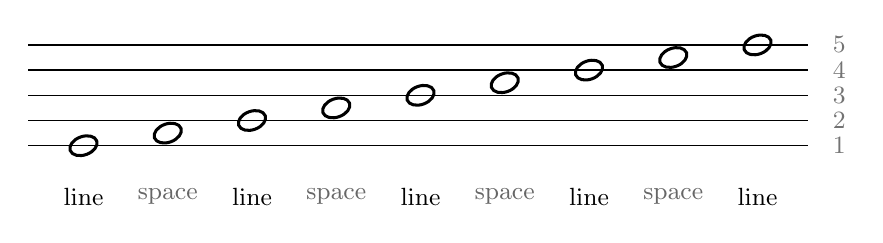
\begin{tikzpicture}
\draw[line width=0.5pt] (0,0) -- (9.9,0);
\draw[line width=0.5pt] (0,0.32) -- (9.9,0.32);
\draw[line width=0.5pt] (0,0.64) -- (9.9,0.64);
\draw[line width=0.5pt] (0,0.96) -- (9.9,0.96);
\draw[line width=0.5pt] (0,1.28) -- (9.9,1.28);
\node[font=\small, text=black!55] at (10.3,0) {1};
\node[font=\small, text=black!55] at (10.3,0.32) {2};
\node[font=\small, text=black!55] at (10.3,0.64) {3};
\node[font=\small, text=black!55] at (10.3,0.96) {4};
\node[font=\small, text=black!55] at (10.3,1.28) {5};
\draw[black, line width=1.1pt, rotate around={20:(0.7,0)}] (0.7,0) ellipse (0.179 and 0.117);
\node[font=\small] at (0.7,-0.65) {line};
\draw[black, line width=1.1pt, rotate around={20:(1.77,0.16)}] (1.77,0.16) ellipse (0.179 and 0.117);
\node[font=\small, text=black!60] at (1.77,-0.65) {space};
\draw[black, line width=1.1pt, rotate around={20:(2.84,0.32)}] (2.84,0.32) ellipse (0.179 and 0.117);
\node[font=\small] at (2.84,-0.65) {line};
\draw[black, line width=1.1pt, rotate around={20:(3.91,0.48)}] (3.91,0.48) ellipse (0.179 and 0.117);
\node[font=\small, text=black!60] at (3.91,-0.65) {space};
\draw[black, line width=1.1pt, rotate around={20:(4.98,0.64)}] (4.98,0.64) ellipse (0.179 and 0.117);
\node[font=\small] at (4.98,-0.65) {line};
\draw[black, line width=1.1pt, rotate around={20:(6.05,0.8)}] (6.05,0.8) ellipse (0.179 and 0.117);
\node[font=\small, text=black!60] at (6.05,-0.65) {space};
\draw[black, line width=1.1pt, rotate around={20:(7.12,0.96)}] (7.12,0.96) ellipse (0.179 and 0.117);
\node[font=\small] at (7.12,-0.65) {line};
\draw[black, line width=1.1pt, rotate around={20:(8.19,1.12)}] (8.19,1.12) ellipse (0.179 and 0.117);
\node[font=\small, text=black!60] at (8.19,-0.65) {space};
\draw[black, line width=1.1pt, rotate around={20:(9.26,1.28)}] (9.26,1.28) ellipse (0.179 and 0.117);
\node[font=\small] at (9.26,-0.65) {line};
\end{tikzpicture}
\caption{A staff has five lines and four spaces. Each note here is one step higher than the one before: line, space, line, space.}
\label{fig:staff-ladder}
\end{figure}

Here is the key idea of this chapter. Each line and each space stands for one white key. Moving up from a line to the very next space (or from a space to the next line) moves up one white key, to the next letter of the musical alphabet. We call that move one \textbf{step}.

So climbing the staff is the same as walking up the white keys: C, D, E, F, G, A, B, C, and so on. Higher on the staff means further right on the keyboard, and higher in sound. A step on the staff counts letters, not keys: it can be a half step on the keyboard (E to F, B to C) or a whole step (C to D).

The black keys do not get their own lines or spaces. They are written with sharp and flat signs, which we meet later in this chapter.

\section{Clefs: which note is which}

A bare staff does not say which letter each line is. That is the job of a \textbf{clef}, a symbol drawn at the start of every staff. A clef marks one line as a particular note. Everything else follows by counting steps.

The \textbf{treble clef} is the tall, curly sign. Its inner curl wraps around line 2, and marks that line as G4, the first G above middle C \listen{G4:2}. That is why it is also called the G clef. The treble staff holds higher notes, usually played by the right hand.

The \textbf{bass clef} looks like a backwards C with two dots. The two dots sit on either side of line 4, and mark that line as F3, the first F below middle C \listen{F3:2}. That is why it is also called the F clef. The bass staff holds lower notes, usually played by the left hand.

\begin{figure}[htbp]
\centering
\begin{tikzpicture}
\draw[line width=0.5pt] (0,0) -- (10.6,0);
\draw[line width=0.5pt] (0,0.3) -- (10.6,0.3);
\draw[line width=0.5pt] (0,0.6) -- (10.6,0.6);
\draw[line width=0.5pt] (0,0.9) -- (10.6,0.9);
\draw[line width=0.5pt] (0,1.2) -- (10.6,1.2);
\draw[black, line width=1.451pt, line cap=round] (0.696,0.426) .. controls (0.696,0.585) and (0.45,0.594) .. (0.444,0.375) .. controls (0.435,0.09) and (0.894,0.054) .. (0.906,0.336) .. controls (0.918,0.615) and (0.57,0.75) .. (0.414,0.93) .. controls (0.27,1.11) and (0.42,1.47) .. (0.66,1.665) .. controls (0.75,1.74) and (0.798,1.59) .. (0.726,1.425) .. controls (0.666,1.29) and (0.594,1.17) .. (0.606,0.9) -- (0.66,-0.255) .. controls (0.672,-0.465) and (0.45,-0.486) .. (0.414,-0.33);
\fill[black] (0.474,-0.306) circle (0.078);
\draw[black, line width=1.1pt, rotate around={20:(1.9,0)}] (1.9,0) ellipse (0.167 and 0.11);
\node[font=\small] at (1.9,-0.6) {E4};
\draw[black, line width=1.1pt, rotate around={20:(2.87,0.15)}] (2.87,0.15) ellipse (0.167 and 0.11);
\node[font=\small] at (2.87,-0.6) {F4};
\draw[sourceblue, line width=1.1pt, rotate around={20:(3.84,0.3)}] (3.84,0.3) ellipse (0.167 and 0.11);
\node[font=\small, text=sourceblue, font=\small\bfseries] at (3.84,-0.6) {G4};
\draw[black, line width=1.1pt, rotate around={20:(4.81,0.45)}] (4.81,0.45) ellipse (0.167 and 0.11);
\node[font=\small] at (4.81,-0.6) {A4};
\draw[black, line width=1.1pt, rotate around={20:(5.78,0.6)}] (5.78,0.6) ellipse (0.167 and 0.11);
\node[font=\small] at (5.78,-0.6) {B4};
\draw[black, line width=1.1pt, rotate around={20:(6.75,0.75)}] (6.75,0.75) ellipse (0.167 and 0.11);
\node[font=\small] at (6.75,-0.6) {C5};
\draw[black, line width=1.1pt, rotate around={20:(7.72,0.9)}] (7.72,0.9) ellipse (0.167 and 0.11);
\node[font=\small] at (7.72,-0.6) {D5};
\draw[black, line width=1.1pt, rotate around={20:(8.69,1.05)}] (8.69,1.05) ellipse (0.167 and 0.11);
\node[font=\small] at (8.69,-0.6) {E5};
\draw[black, line width=1.1pt, rotate around={20:(9.66,1.2)}] (9.66,1.2) ellipse (0.167 and 0.11);
\node[font=\small] at (9.66,-0.6) {F5};
\draw[line width=0.5pt] (0,-3.1) -- (10.6,-3.1);
\draw[line width=0.5pt] (0,-2.8) -- (10.6,-2.8);
\draw[line width=0.5pt] (0,-2.5) -- (10.6,-2.5);
\draw[line width=0.5pt] (0,-2.2) -- (10.6,-2.2);
\draw[line width=0.5pt] (0,-1.9) -- (10.6,-1.9);
\draw[black, line width=1.707pt, line cap=round] (0.39,-2.2) .. controls (0.405,-1.915) and (0.855,-1.855) .. (0.876,-2.215) .. controls (0.894,-2.575) and (0.57,-2.86) .. (0.285,-3.01);
\fill[black] (0.39,-2.2) circle (0.09);
\fill[black] (1.005,-2.05) circle (0.048);
\fill[black] (1.005,-2.35) circle (0.048);
\draw[black, line width=1.1pt, rotate around={20:(1.9,-3.1)}] (1.9,-3.1) ellipse (0.167 and 0.11);
\node[font=\small] at (1.9,-3.7) {G2};
\draw[black, line width=1.1pt, rotate around={20:(2.87,-2.95)}] (2.87,-2.95) ellipse (0.167 and 0.11);
\node[font=\small] at (2.87,-3.7) {A2};
\draw[black, line width=1.1pt, rotate around={20:(3.84,-2.8)}] (3.84,-2.8) ellipse (0.167 and 0.11);
\node[font=\small] at (3.84,-3.7) {B2};
\draw[black, line width=1.1pt, rotate around={20:(4.81,-2.65)}] (4.81,-2.65) ellipse (0.167 and 0.11);
\node[font=\small] at (4.81,-3.7) {C3};
\draw[black, line width=1.1pt, rotate around={20:(5.78,-2.5)}] (5.78,-2.5) ellipse (0.167 and 0.11);
\node[font=\small] at (5.78,-3.7) {D3};
\draw[black, line width=1.1pt, rotate around={20:(6.75,-2.35)}] (6.75,-2.35) ellipse (0.167 and 0.11);
\node[font=\small] at (6.75,-3.7) {E3};
\draw[sourceblue, line width=1.1pt, rotate around={20:(7.72,-2.2)}] (7.72,-2.2) ellipse (0.167 and 0.11);
\node[font=\small, text=sourceblue, font=\small\bfseries] at (7.72,-3.7) {F3};
\draw[black, line width=1.1pt, rotate around={20:(8.69,-2.05)}] (8.69,-2.05) ellipse (0.167 and 0.11);
\node[font=\small] at (8.69,-3.7) {G3};
\draw[black, line width=1.1pt, rotate around={20:(9.66,-1.9)}] (9.66,-1.9) ellipse (0.167 and 0.11);
\node[font=\small] at (9.66,-3.7) {A3};
\end{tikzpicture}
\caption{The treble clef marks G4 (line 2) and the bass clef marks F3 (line 4). Every other line and space follows by stepping up or down.}
\label{fig:clefs}
\end{figure}

From those two notes you can fill in the rest by stepping, as in Figure~\ref{fig:clefs}.
\begin{itemize}
  \item Treble staff, lines from the bottom: E4, G4, B4, D5, F5 \listen{E4 G4 B4 D5 F5:2}. Spaces: F4, A4, C5, E5 \listen{F4 A4 C5 E5:2}.
  \item Bass staff, lines from the bottom: G2, B2, D3, F3, A3 \listen{G2 B2 D3 F3 A3:2}. Spaces: A2, C3, E3, G3 \listen{A2 C3 E3 G3:2}.
\end{itemize}

You may have heard rhymes for these, like ``Every Good Boy Does Fine'' for the treble lines and ``FACE'' for the treble spaces. They work, but reciting a rhyme for every note is slow. The landmark method below is quicker once it clicks, and you can always fall back on a rhyme.

\section{The grand staff and middle C}

Piano music uses two staves at once, joined at the left by a long line or a curly bracket. Together they are called the \textbf{grand staff}: treble on top for the right hand, bass below for the left hand.

The two staves fit together like one tall ladder. The top line of the bass staff is A3. One step up is B3, in the space directly above it. One more step up is middle C, C4. One more step is D4, in the space directly below the treble staff. And one more step lands on E4, the bottom line of the treble staff.

Middle C sits between the two staves, so it gets its own short line drawn through it. A short line like this, added above or below a staff, is called a \textbf{ledger line}. Figure~\ref{fig:grand-staff} shows middle C on its ledger line, halfway between the staves \listen{C4:2}.

\begin{figure}[htbp]
\centering
\begin{tikzpicture}
\draw[line width=0.5pt] (0,1.56) -- (10.6,1.56);
\draw[line width=0.5pt] (0,1.82) -- (10.6,1.82);
\draw[line width=0.5pt] (0,2.08) -- (10.6,2.08);
\draw[line width=0.5pt] (0,2.34) -- (10.6,2.34);
\draw[line width=0.5pt] (0,2.6) -- (10.6,2.6);
\draw[line width=0.5pt] (0,0) -- (10.6,0);
\draw[line width=0.5pt] (0,0.26) -- (10.6,0.26);
\draw[line width=0.5pt] (0,0.52) -- (10.6,0.52);
\draw[line width=0.5pt] (0,0.78) -- (10.6,0.78);
\draw[line width=0.5pt] (0,1.04) -- (10.6,1.04);
\draw[line width=1.2pt] (0,0) -- (0,2.6);
\draw[black, line width=1.257pt, line cap=round] (0.733,1.929) .. controls (0.733,2.067) and (0.52,2.075) .. (0.515,1.885) .. controls (0.507,1.638) and (0.905,1.607) .. (0.915,1.851) .. controls (0.926,2.093) and (0.624,2.21) .. (0.489,2.366) .. controls (0.364,2.522) and (0.494,2.834) .. (0.702,3.003) .. controls (0.78,3.068) and (0.822,2.938) .. (0.759,2.795) .. controls (0.707,2.678) and (0.645,2.574) .. (0.655,2.34) -- (0.702,1.339) .. controls (0.712,1.157) and (0.52,1.139) .. (0.489,1.274);
\fill[black] (0.541,1.295) circle (0.068);
\draw[black, line width=1.479pt, line cap=round] (0.468,0.78) .. controls (0.481,1.027) and (0.871,1.079) .. (0.889,0.767) .. controls (0.905,0.455) and (0.624,0.208) .. (0.377,0.078);
\fill[black] (0.468,0.78) circle (0.078);
\fill[black] (1.001,0.91) circle (0.042);
\fill[black] (1.001,0.65) circle (0.042);
\draw[black, line width=0.6pt] (1.927,-0.26) -- (2.473,-0.26);
\draw[black, line width=0.6pt] (1.927,-0.52) -- (2.473,-0.52);
\draw[black, line width=1.1pt, rotate around={20:(2.2,-0.52)}] (2.2,-0.52) ellipse (0.145 and 0.095);
\node[font=\small] at (2.2,-1.27) {C2};
\draw[black, line width=1.1pt, rotate around={20:(3.5,0.39)}] (3.5,0.39) ellipse (0.145 and 0.095);
\node[font=\small] at (3.5,-1.27) {C3};
\draw[black, line width=1.1pt, rotate around={20:(4.8,0.78)}] (4.8,0.78) ellipse (0.145 and 0.095);
\node[font=\small] at (4.8,-1.27) {F3};
\draw[black, line width=0.6pt] (5.827,1.3) -- (6.373,1.3);
\draw[quotientorange!90!black, line width=1.1pt, rotate around={20:(6.1,1.3)}] (6.1,1.3) ellipse (0.145 and 0.095);
\node[font=\small, font=\small\bfseries] at (6.1,-1.27) {C4};
\draw[black, line width=1.1pt, rotate around={20:(7.4,1.82)}] (7.4,1.82) ellipse (0.145 and 0.095);
\node[font=\small] at (7.4,-1.27) {G4};
\draw[black, line width=1.1pt, rotate around={20:(8.7,2.21)}] (8.7,2.21) ellipse (0.145 and 0.095);
\node[font=\small] at (8.7,-1.27) {C5};
\draw[black, line width=0.6pt] (9.727,2.86) -- (10.273,2.86);
\draw[black, line width=0.6pt] (9.727,3.12) -- (10.273,3.12);
\draw[black, line width=1.1pt, rotate around={20:(10,3.12)}] (10,3.12) ellipse (0.145 and 0.095);
\node[font=\small] at (10,-1.27) {C6};
\end{tikzpicture}
\caption{The grand staff, drawn as one ladder. Middle C (C4) sits on its own ledger line between the staves. The other notes shown are the landmarks of the next section.}
\label{fig:grand-staff}
\end{figure}

In printed music the two staves are drawn further apart, to leave room. Then middle C appears in one of two places: on a ledger line directly below the treble staff when the right hand plays it, or directly above the bass staff when the left hand plays it. Both are the same key, as Figure~\ref{fig:printed-c} shows.

\begin{figure}[htbp]
\centering
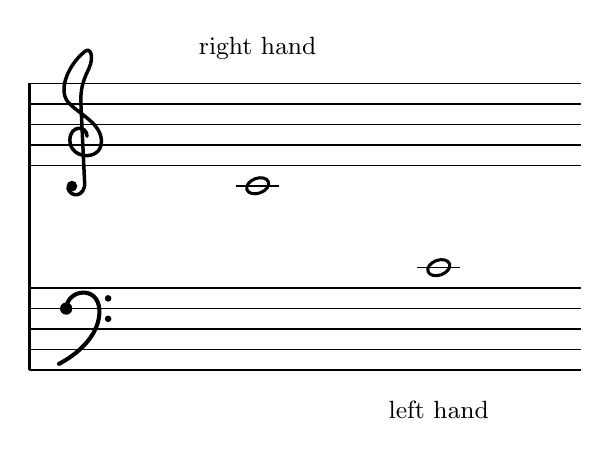
\begin{tikzpicture}
\draw[line width=0.5pt] (0,2.6) -- (7,2.6);
\draw[line width=0.5pt] (0,2.86) -- (7,2.86);
\draw[line width=0.5pt] (0,3.12) -- (7,3.12);
\draw[line width=0.5pt] (0,3.38) -- (7,3.38);
\draw[line width=0.5pt] (0,3.64) -- (7,3.64);
\draw[line width=0.5pt] (0,0) -- (7,0);
\draw[line width=0.5pt] (0,0.26) -- (7,0.26);
\draw[line width=0.5pt] (0,0.52) -- (7,0.52);
\draw[line width=0.5pt] (0,0.78) -- (7,0.78);
\draw[line width=0.5pt] (0,1.04) -- (7,1.04);
\draw[line width=1.2pt] (0,0) -- (0,3.64);
\draw[black, line width=1.257pt, line cap=round] (0.733,2.969) .. controls (0.733,3.107) and (0.52,3.115) .. (0.515,2.925) .. controls (0.507,2.678) and (0.905,2.647) .. (0.915,2.891) .. controls (0.926,3.133) and (0.624,3.25) .. (0.489,3.406) .. controls (0.364,3.562) and (0.494,3.874) .. (0.702,4.043) .. controls (0.78,4.108) and (0.822,3.978) .. (0.759,3.835) .. controls (0.707,3.718) and (0.645,3.614) .. (0.655,3.38) -- (0.702,2.379) .. controls (0.712,2.197) and (0.52,2.179) .. (0.489,2.314);
\fill[black] (0.541,2.335) circle (0.068);
\draw[black, line width=1.479pt, line cap=round] (0.468,0.78) .. controls (0.481,1.027) and (0.871,1.079) .. (0.889,0.767) .. controls (0.905,0.455) and (0.624,0.208) .. (0.377,0.078);
\fill[black] (0.468,0.78) circle (0.078);
\fill[black] (1.001,0.91) circle (0.042);
\fill[black] (1.001,0.65) circle (0.042);
\draw[black, line width=0.6pt] (2.627,2.34) -- (3.173,2.34);
\draw[black, line width=1.1pt, rotate around={20:(2.9,2.34)}] (2.9,2.34) ellipse (0.145 and 0.095);
\draw[black, line width=0.6pt] (4.927,1.3) -- (5.473,1.3);
\draw[black, line width=1.1pt, rotate around={20:(5.2,1.3)}] (5.2,1.3) ellipse (0.145 and 0.095);
\node[font=\small] at (2.9,4.09) {right hand};
\node[font=\small] at (5.2,-0.5) {left hand};
\end{tikzpicture}
\caption{In printed music, middle C is written directly below the treble staff (for the right hand) or directly above the bass staff (for the left hand). Both mean the same key.}
\label{fig:printed-c}
\end{figure}

\section{Ledger lines}

Ledger lines work the same way above and below any staff. They extend the ladder: each extra short line is one more line of the staff, and the spaces between them count too.

Above the treble staff: the top line is F5. The space above it is G5, then A5 sits on the first ledger line, B5 above it, and C6 on the second ledger line \listen{F5 G5 A5 B5 C6:2}. Below the treble staff: D4 hangs directly under the bottom line, then C4 on one ledger line, then B3 and A3 \listen{D4 C4 B3 A3:2}.

The bass staff works the same way. Below its bottom line (G2) come F2, then E2 on the first ledger line, D2, and C2 on the second ledger line \listen{G2 F2 E2 D2 C2:2}.

\begin{figure}[htbp]
\centering
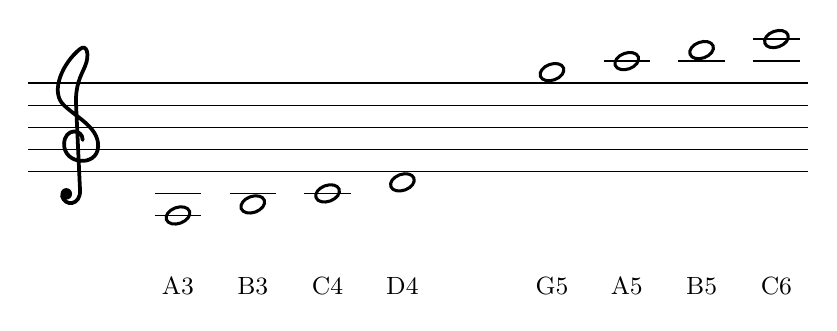
\begin{tikzpicture}
\draw[line width=0.5pt] (0,0) -- (9.9,0);
\draw[line width=0.5pt] (0,0.28) -- (9.9,0.28);
\draw[line width=0.5pt] (0,0.56) -- (9.9,0.56);
\draw[line width=0.5pt] (0,0.84) -- (9.9,0.84);
\draw[line width=0.5pt] (0,1.12) -- (9.9,1.12);
\draw[black, line width=1.354pt, line cap=round] (0.69,0.398) .. controls (0.69,0.546) and (0.46,0.554) .. (0.454,0.35) .. controls (0.446,0.084) and (0.874,0.05) .. (0.886,0.314) .. controls (0.897,0.574) and (0.572,0.7) .. (0.426,0.868) .. controls (0.292,1.036) and (0.432,1.372) .. (0.656,1.554) .. controls (0.74,1.624) and (0.785,1.484) .. (0.718,1.33) .. controls (0.662,1.204) and (0.594,1.092) .. (0.606,0.84) -- (0.656,-0.238) .. controls (0.667,-0.434) and (0.46,-0.454) .. (0.426,-0.308);
\fill[black] (0.482,-0.286) circle (0.073);
\draw[black, line width=0.6pt] (1.606,-0.28) -- (2.194,-0.28);
\draw[black, line width=0.6pt] (1.606,-0.56) -- (2.194,-0.56);
\draw[black, line width=1.1pt, rotate around={20:(1.9,-0.56)}] (1.9,-0.56) ellipse (0.156 and 0.102);
\node[font=\small] at (1.9,-1.45) {A3};
\draw[black, line width=0.6pt] (2.556,-0.28) -- (3.144,-0.28);
\draw[black, line width=1.1pt, rotate around={20:(2.85,-0.42)}] (2.85,-0.42) ellipse (0.156 and 0.102);
\node[font=\small] at (2.85,-1.45) {B3};
\draw[black, line width=0.6pt] (3.506,-0.28) -- (4.094,-0.28);
\draw[black, line width=1.1pt, rotate around={20:(3.8,-0.28)}] (3.8,-0.28) ellipse (0.156 and 0.102);
\node[font=\small] at (3.8,-1.45) {C4};
\draw[black, line width=1.1pt, rotate around={20:(4.75,-0.14)}] (4.75,-0.14) ellipse (0.156 and 0.102);
\node[font=\small] at (4.75,-1.45) {D4};
\draw[black, line width=1.1pt, rotate around={20:(6.65,1.26)}] (6.65,1.26) ellipse (0.156 and 0.102);
\node[font=\small] at (6.65,-1.45) {G5};
\draw[black, line width=0.6pt] (7.306,1.4) -- (7.894,1.4);
\draw[black, line width=1.1pt, rotate around={20:(7.6,1.4)}] (7.6,1.4) ellipse (0.156 and 0.102);
\node[font=\small] at (7.6,-1.45) {A5};
\draw[black, line width=0.6pt] (8.256,1.4) -- (8.844,1.4);
\draw[black, line width=1.1pt, rotate around={20:(8.55,1.54)}] (8.55,1.54) ellipse (0.156 and 0.102);
\node[font=\small] at (8.55,-1.45) {B5};
\draw[black, line width=0.6pt] (9.206,1.4) -- (9.794,1.4);
\draw[black, line width=0.6pt] (9.206,1.68) -- (9.794,1.68);
\draw[black, line width=1.1pt, rotate around={20:(9.5,1.68)}] (9.5,1.68) ellipse (0.156 and 0.102);
\node[font=\small] at (9.5,-1.45) {C6};
\end{tikzpicture}
\caption{Ledger lines extend the treble staff downward (A3 to D4) and upward (G5 to C6). Count them like ordinary lines and spaces.}
\label{fig:ledger}
\end{figure}

\section{Landmark notes}

Reading music fluently does not mean naming every note from scratch. It means knowing a handful of landmark notes by sight, and counting a step or two from the nearest one.

Here are five landmarks, all around middle C (they are in Figure~\ref{fig:grand-staff}):
\begin{itemize}
  \item Middle C (C4), on its own ledger line between the staves \listen{C4:2}.
  \item G4, the treble clef line (line 2 of the treble staff) \listen{G4:2}.
  \item F3, the bass clef line (line 4 of the bass staff) \listen{F3:2}.
  \item C5, in space 3 of the treble staff \listen{C5:2}.
  \item C3, in space 2 of the bass staff \listen{C3:2}.
\end{itemize}

Notice the mirror pattern. G4 is the second line up from the bottom of the treble staff; F3 is the second line down from the top of the bass staff. Both sit four steps away from middle C, one above and one below. C5 and C3 sit seven steps away, again one above and one below.

Hear the five landmarks from low to high \listen{C3 F3 C4 G4 C5:2}.

From C3 up to C5, every white key is at most two steps from one of these five landmarks. To read a note, find the nearest landmark and count. One step goes from a line to the next space (or a space to the next line). Two steps go from a line to the next line, or from a space to the next space.

For notes further out, add four more landmarks: the bottom line of the bass staff (G2), the top line of the treble staff (F5), and the two Cs on second ledger lines, C2 below the bass staff and C6 above the treble staff \listen{C2 G2 F5 C6:2}. With all nine, every white key from C2 up to C6 is within two steps of a landmark.

A few examples:
\begin{itemize}
  \item The next treble line above G4 is two steps up (G, A, B), so it is B4 \listen{G4 B4:2}.
  \item The space directly above middle C is one step up, so it is D4 \listen{C4 D4:2}.
  \item The next bass line below F3 is two steps down (F, E, D), so it is D3 \listen{F3 D3:2}.
\end{itemize}

\begin{tryitbox}
Put the thumb of your right hand on middle C and look at Figure~\ref{fig:grand-staff}. Play C4, then G4 with your little finger. Then put your left little finger on C3 and play F3 with your index finger (finger 2), then C3 again. Say each landmark's name out loud as you play it.
\end{tryitbox}

\section{Sharps, flats and naturals on paper}

Black keys are written with signs placed directly before the note, on the same line or space.
\begin{itemize}
  \item A \textbf{sharp} sign (\sh) means: play the key one half step higher. A note on the F4 space with a sharp is F\sh4, the black key directly right of F4 \listen{F4 F#4:2}.
  \item A \textbf{flat} sign (\fl) means: play the key one half step lower. A note on the B4 line with a flat is B\fl4, the black key directly left of B4 \listen{B4 Bb4:2}.
  \item A \textbf{natural} sign (\nat) cancels a sharp or flat and brings the note back to the white key \listen{F#4 F4:2}.
\end{itemize}

A sharp, flat or natural written in front of a note is called an \textbf{accidental}. It lasts until the end of the bar, for every note on that same line or space. At the next bar line it is forgotten.

\begin{figure}[htbp]
\centering
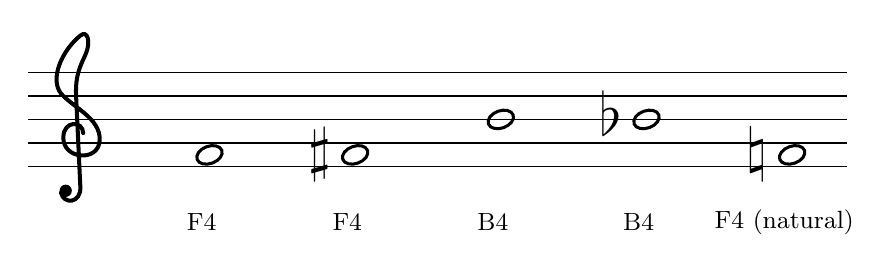
\begin{tikzpicture}
\draw[line width=0.5pt] (0,0) -- (10.4,0);
\draw[line width=0.5pt] (0,0.3) -- (10.4,0.3);
\draw[line width=0.5pt] (0,0.6) -- (10.4,0.6);
\draw[line width=0.5pt] (0,0.9) -- (10.4,0.9);
\draw[line width=0.5pt] (0,1.2) -- (10.4,1.2);
\draw[black, line width=1.451pt, line cap=round] (0.696,0.426) .. controls (0.696,0.585) and (0.45,0.594) .. (0.444,0.375) .. controls (0.435,0.09) and (0.894,0.054) .. (0.906,0.336) .. controls (0.918,0.615) and (0.57,0.75) .. (0.414,0.93) .. controls (0.27,1.11) and (0.42,1.47) .. (0.66,1.665) .. controls (0.75,1.74) and (0.798,1.59) .. (0.726,1.425) .. controls (0.666,1.29) and (0.594,1.17) .. (0.606,0.9) -- (0.66,-0.255) .. controls (0.672,-0.465) and (0.45,-0.486) .. (0.414,-0.33);
\fill[black] (0.474,-0.306) circle (0.078);
\draw[black, line width=1.1pt, rotate around={20:(2.3,0.15)}] (2.3,0.15) ellipse (0.167 and 0.11);
\node[font=\small] at (2.2,-0.7) {F4};
\node[black, font=\Large, scale=1.5, inner sep=0] at (3.7,0.15) {$\sharp$};
\draw[black, line width=1.1pt, rotate around={20:(4.15,0.15)}] (4.15,0.15) ellipse (0.167 and 0.11);
\node[font=\small] at (4.05,-0.7) {F\sh4};
\draw[black, line width=1.1pt, rotate around={20:(6,0.6)}] (6,0.6) ellipse (0.167 and 0.11);
\node[font=\small] at (5.9,-0.7) {B4};
\node[black, font=\Large, scale=1.5, inner sep=0] at (7.4,0.675) {$\flat$};
\draw[black, line width=1.1pt, rotate around={20:(7.85,0.6)}] (7.85,0.6) ellipse (0.167 and 0.11);
\node[font=\small] at (7.75,-0.7) {B\fl4};
\node[black, font=\Large, scale=1.5, inner sep=0] at (9.25,0.15) {$\natural$};
\draw[black, line width=1.1pt, rotate around={20:(9.7,0.15)}] (9.7,0.15) ellipse (0.167 and 0.11);
\node[font=\small] at (9.6,-0.7) {F4 (natural)};
\end{tikzpicture}
\caption{A sharp raises a note by a half step, a flat lowers it by a half step, and a natural cancels either one.}
\label{fig:accidentals}
\end{figure}

\section{Key signatures}

Chapter~\ref{ch:scales-and-keys} showed that the scale of G major uses F\sh{} instead of F. A piece in the key of G (a piece built on that scale) would need a sharp in front of every F. Writing them all out would be tiring.

Instead, the sharps or flats a piece needs are written once, at the start of every staff, directly after the clef. This group is called the \textbf{key signature}. A sharp on the F line in the key signature means: every F in the piece, in every octave, is played as F\sh, unless a natural sign says otherwise.

Figure~\ref{fig:key-signatures} shows four key signatures. The sharps always appear in the same order, F C G D A E B, and the flats in the order B E A D G C F, as in Chapter~\ref{ch:scales-and-keys}.

\begin{figure}[htbp]
\centering
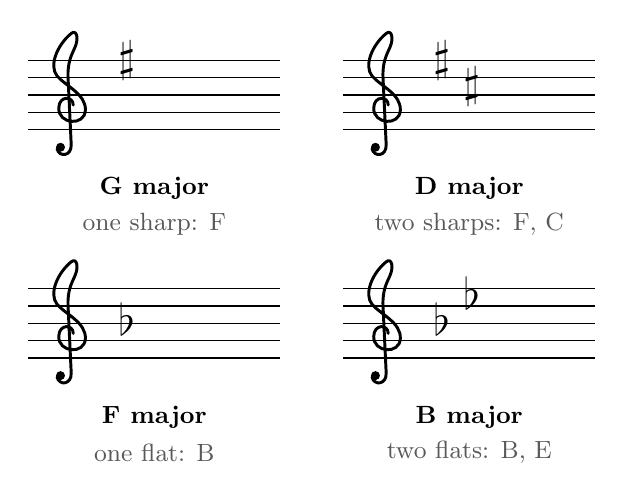
\begin{tikzpicture}
\draw[line width=0.5pt] (0,0) -- (3.2,0);
\draw[line width=0.5pt] (0,0.22) -- (3.2,0.22);
\draw[line width=0.5pt] (0,0.44) -- (3.2,0.44);
\draw[line width=0.5pt] (0,0.66) -- (3.2,0.66);
\draw[line width=0.5pt] (0,0.88) -- (3.2,0.88);
\draw[black, line width=1.064pt, line cap=round] (0.57,0.312) .. controls (0.57,0.429) and (0.39,0.436) .. (0.386,0.275) .. controls (0.379,0.066) and (0.716,0.04) .. (0.724,0.246) .. controls (0.733,0.451) and (0.478,0.55) .. (0.364,0.682) .. controls (0.258,0.814) and (0.368,1.078) .. (0.544,1.221) .. controls (0.61,1.276) and (0.645,1.166) .. (0.592,1.045) .. controls (0.548,0.946) and (0.496,0.858) .. (0.504,0.66) -- (0.544,-0.187) .. controls (0.553,-0.341) and (0.39,-0.356) .. (0.364,-0.242);
\fill[black] (0.408,-0.224) circle (0.057);
\node[black, font=\Large, scale=1.1, inner sep=0] at (1.25,0.88) {$\sharp$};
\node[font=\small, font=\small\bfseries] at (1.6,-0.75) {G major};
\node[font=\small, text=black!65] at (1.6,-1.2) {one sharp: F\sh};
\draw[line width=0.5pt] (4,0) -- (7.2,0);
\draw[line width=0.5pt] (4,0.22) -- (7.2,0.22);
\draw[line width=0.5pt] (4,0.44) -- (7.2,0.44);
\draw[line width=0.5pt] (4,0.66) -- (7.2,0.66);
\draw[line width=0.5pt] (4,0.88) -- (7.2,0.88);
\draw[black, line width=1.064pt, line cap=round] (4.57,0.312) .. controls (4.57,0.429) and (4.39,0.436) .. (4.386,0.275) .. controls (4.379,0.066) and (4.716,0.04) .. (4.724,0.246) .. controls (4.733,0.451) and (4.478,0.55) .. (4.364,0.682) .. controls (4.258,0.814) and (4.368,1.078) .. (4.544,1.221) .. controls (4.61,1.276) and (4.645,1.166) .. (4.592,1.045) .. controls (4.548,0.946) and (4.496,0.858) .. (4.504,0.66) -- (4.544,-0.187) .. controls (4.553,-0.341) and (4.39,-0.356) .. (4.364,-0.242);
\fill[black] (4.408,-0.224) circle (0.057);
\node[black, font=\Large, scale=1.1, inner sep=0] at (5.25,0.88) {$\sharp$};
\node[black, font=\Large, scale=1.1, inner sep=0] at (5.63,0.55) {$\sharp$};
\node[font=\small, font=\small\bfseries] at (5.6,-0.75) {D major};
\node[font=\small, text=black!65] at (5.6,-1.2) {two sharps: F\sh, C\sh};
\draw[line width=0.5pt] (0,-2.9) -- (3.2,-2.9);
\draw[line width=0.5pt] (0,-2.68) -- (3.2,-2.68);
\draw[line width=0.5pt] (0,-2.46) -- (3.2,-2.46);
\draw[line width=0.5pt] (0,-2.24) -- (3.2,-2.24);
\draw[line width=0.5pt] (0,-2.02) -- (3.2,-2.02);
\draw[black, line width=1.064pt, line cap=round] (0.57,-2.588) .. controls (0.57,-2.471) and (0.39,-2.464) .. (0.386,-2.625) .. controls (0.379,-2.834) and (0.716,-2.86) .. (0.724,-2.654) .. controls (0.733,-2.449) and (0.478,-2.35) .. (0.364,-2.218) .. controls (0.258,-2.086) and (0.368,-1.822) .. (0.544,-1.679) .. controls (0.61,-1.624) and (0.645,-1.734) .. (0.592,-1.855) .. controls (0.548,-1.954) and (0.496,-2.042) .. (0.504,-2.24) -- (0.544,-3.087) .. controls (0.553,-3.241) and (0.39,-3.256) .. (0.364,-3.142);
\fill[black] (0.408,-3.124) circle (0.057);
\node[black, font=\Large, scale=1.1, inner sep=0] at (1.25,-2.405) {$\flat$};
\node[font=\small, font=\small\bfseries] at (1.6,-3.65) {F major};
\node[font=\small, text=black!65] at (1.6,-4.1) {one flat: B\fl};
\draw[line width=0.5pt] (4,-2.9) -- (7.2,-2.9);
\draw[line width=0.5pt] (4,-2.68) -- (7.2,-2.68);
\draw[line width=0.5pt] (4,-2.46) -- (7.2,-2.46);
\draw[line width=0.5pt] (4,-2.24) -- (7.2,-2.24);
\draw[line width=0.5pt] (4,-2.02) -- (7.2,-2.02);
\draw[black, line width=1.064pt, line cap=round] (4.57,-2.588) .. controls (4.57,-2.471) and (4.39,-2.464) .. (4.386,-2.625) .. controls (4.379,-2.834) and (4.716,-2.86) .. (4.724,-2.654) .. controls (4.733,-2.449) and (4.478,-2.35) .. (4.364,-2.218) .. controls (4.258,-2.086) and (4.368,-1.822) .. (4.544,-1.679) .. controls (4.61,-1.624) and (4.645,-1.734) .. (4.592,-1.855) .. controls (4.548,-1.954) and (4.496,-2.042) .. (4.504,-2.24) -- (4.544,-3.087) .. controls (4.553,-3.241) and (4.39,-3.256) .. (4.364,-3.142);
\fill[black] (4.408,-3.124) circle (0.057);
\node[black, font=\Large, scale=1.1, inner sep=0] at (5.25,-2.405) {$\flat$};
\node[black, font=\Large, scale=1.1, inner sep=0] at (5.63,-2.075) {$\flat$};
\node[font=\small, font=\small\bfseries] at (5.6,-3.65) {B\fl{} major};
\node[font=\small, text=black!65] at (5.6,-4.1) {two flats: B\fl, E\fl};
\end{tikzpicture}
\caption{Four key signatures on the treble staff. The signs sit on the lines and spaces of the notes they change.}
\label{fig:key-signatures}
\end{figure}

Two quick tricks tell you the key:
\begin{itemize}
  \item \emph{Sharps:} take the last sharp and go up one half step. One sharp (F\sh): up a half step is G, so G major \listen{G4 A4 B4 C5 D5 E5 F#5 G5:2}. Two sharps (F\sh, C\sh): the last is C\sh, up a half step is D, so D major \listen{D4 E4 F#4 G4 A4 B4 C#5 D5:2}.
  \item \emph{Flats:} the second-to-last flat is the key. Two flats (B\fl, E\fl): the second-to-last is B\fl, so B\fl{} major \listen{Bb3 C4 D4 Eb4 F4 G4 A4 Bb4:2}. One flat has no second-to-last, so learn that one by heart: one flat (B\fl) means F major \listen{F4 G4 A4 Bb4 C5 D5 E5 F5:2}.
\end{itemize}
No sharps or flats at all means C major.

Each key signature is also shared by one minor key, its relative minor from Chapter~\ref{ch:scales-and-keys}. To find it, count down three half steps from the major key's name. G major and E minor share one sharp; C major and A minor share no sharps or flats. The last note of a piece usually tells you which one it is: a piece in E minor tends to end on E.

\section{Intervals by shape}

In Chapter~\ref{ch:keyboard-geometry} you measured an \emph{interval}, the distance between two notes, in half steps. On the staff it is named by counting letters, including both ends. C up to E is a third, because it covers three letters: C, D, E.

The staff shows intervals as shapes, so you can read them without naming the notes. Figure~\ref{fig:intervals} shows the common ones, all starting from E4 on the bottom line.
\begin{itemize}
  \item A step (a second) goes from a line to the very next space, or a space to the next line \listen{E4 F4}.
  \item A \textbf{skip} (a third) goes from a line to the next line, or a space to the next space \listen{E4 G4}.
  \item A fourth goes from a line to the second space above it \listen{E4 A4}.
  \item A fifth goes from a line to a line two away, skipping one line in between \listen{E4 B4}.
  \item An octave (an eighth) goes from E to the next E, from a line to a space \listen{E4 E5}.
\end{itemize}

There is a handy pattern. Odd intervals (third, fifth, seventh) go from a line to a line, or a space to a space. Even intervals (second, fourth, sixth, octave) switch between line and space.

\begin{figure}[htbp]
\centering
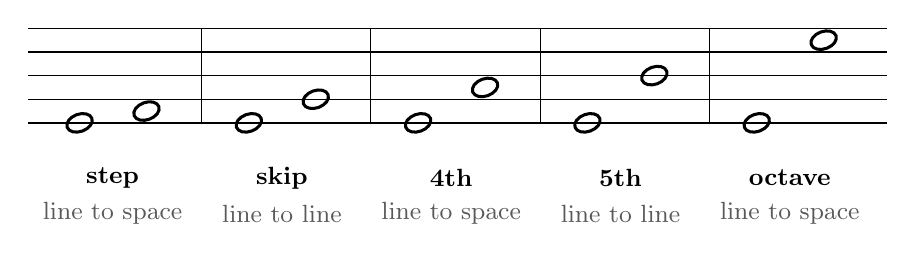
\begin{tikzpicture}
\draw[line width=0.5pt] (0,0) -- (10.9,0);
\draw[line width=0.5pt] (0,0.3) -- (10.9,0.3);
\draw[line width=0.5pt] (0,0.6) -- (10.9,0.6);
\draw[line width=0.5pt] (0,0.9) -- (10.9,0.9);
\draw[line width=0.5pt] (0,1.2) -- (10.9,1.2);
\draw[black, line width=1.1pt, rotate around={20:(0.65,0)}] (0.65,0) ellipse (0.167 and 0.11);
\draw[black, line width=1.1pt, rotate around={20:(1.5,0.15)}] (1.5,0.15) ellipse (0.167 and 0.11);
\node[font=\small, font=\small\bfseries] at (1.07,-0.7) {step};
\node[font=\small, text=black!65] at (1.07,-1.15) {line to space};
\draw[line width=0.4pt] (2.2,0) -- (2.2,1.2);
\draw[black, line width=1.1pt, rotate around={20:(2.8,0)}] (2.8,0) ellipse (0.167 and 0.11);
\draw[black, line width=1.1pt, rotate around={20:(3.65,0.3)}] (3.65,0.3) ellipse (0.167 and 0.11);
\node[font=\small, font=\small\bfseries] at (3.22,-0.7) {skip};
\node[font=\small, text=black!65] at (3.22,-1.15) {line to line};
\draw[line width=0.4pt] (4.35,0) -- (4.35,1.2);
\draw[black, line width=1.1pt, rotate around={20:(4.95,0)}] (4.95,0) ellipse (0.167 and 0.11);
\draw[black, line width=1.1pt, rotate around={20:(5.8,0.45)}] (5.8,0.45) ellipse (0.167 and 0.11);
\node[font=\small, font=\small\bfseries] at (5.37,-0.7) {4th};
\node[font=\small, text=black!65] at (5.37,-1.15) {line to space};
\draw[line width=0.4pt] (6.5,0) -- (6.5,1.2);
\draw[black, line width=1.1pt, rotate around={20:(7.1,0)}] (7.1,0) ellipse (0.167 and 0.11);
\draw[black, line width=1.1pt, rotate around={20:(7.95,0.6)}] (7.95,0.6) ellipse (0.167 and 0.11);
\node[font=\small, font=\small\bfseries] at (7.52,-0.7) {5th};
\node[font=\small, text=black!65] at (7.52,-1.15) {line to line};
\draw[line width=0.4pt] (8.65,0) -- (8.65,1.2);
\draw[black, line width=1.1pt, rotate around={20:(9.25,0)}] (9.25,0) ellipse (0.167 and 0.11);
\draw[black, line width=1.1pt, rotate around={20:(10.1,1.05)}] (10.1,1.05) ellipse (0.167 and 0.11);
\node[font=\small, font=\small\bfseries] at (9.67,-0.7) {octave};
\node[font=\small, text=black!65] at (9.67,-1.15) {line to space};
\end{tikzpicture}
\caption{Intervals as shapes: a step, a skip, a fourth, a fifth and an octave, each starting from E4 on the bottom line.}
\label{fig:intervals}
\end{figure}

This links directly to your fingers. With one finger on each of five neighboring white keys, a step moves to the next finger, a skip skips one finger, and a fifth goes from thumb to little finger. Once your hand is in place, you can read a melody by its ups and downs alone.

\section{Chord shapes on the staff}

A chord written on the staff is a stack of noteheads, one above the other, to be played together. The three positions of a chord from Chapter~\ref{ch:inversions-and-voice-leading} each have their own shape, as Figure~\ref{fig:staff-chords} shows.
\begin{itemize}
  \item \emph{Root position} (C--E--G) stacks on three lines in a row, or three spaces in a row. It looks like a neat snowman \listen{C4+E4+G4:2}.
  \item \emph{First inversion} (E--G--C) has two notes close together at the bottom and a wider gap on top \listen{E4+G4+C5:2}.
  \item \emph{Second inversion} (G--C--E) has a wider gap at the bottom and two notes close together on top \listen{G4+C5+E5:2}.
\end{itemize}

The gap tells you where the root is. In both inversions, the root (the note the chord is named after) is the note directly above the gap.

\begin{figure}[htbp]
\centering
\begin{tikzpicture}
\draw[line width=0.5pt] (0,0) -- (9.6,0);
\draw[line width=0.5pt] (0,0.3) -- (9.6,0.3);
\draw[line width=0.5pt] (0,0.6) -- (9.6,0.6);
\draw[line width=0.5pt] (0,0.9) -- (9.6,0.9);
\draw[line width=0.5pt] (0,1.2) -- (9.6,1.2);
\draw[black, line width=1.451pt, line cap=round] (0.696,0.426) .. controls (0.696,0.585) and (0.45,0.594) .. (0.444,0.375) .. controls (0.435,0.09) and (0.894,0.054) .. (0.906,0.336) .. controls (0.918,0.615) and (0.57,0.75) .. (0.414,0.93) .. controls (0.27,1.11) and (0.42,1.47) .. (0.66,1.665) .. controls (0.75,1.74) and (0.798,1.59) .. (0.726,1.425) .. controls (0.666,1.29) and (0.594,1.17) .. (0.606,0.9) -- (0.66,-0.255) .. controls (0.672,-0.465) and (0.45,-0.486) .. (0.414,-0.33);
\fill[black] (0.474,-0.306) circle (0.078);
\draw[black, line width=0.6pt] (2.285,-0.3) -- (2.915,-0.3);
\draw[quotientorange!90!black, line width=1.1pt, rotate around={20:(2.6,-0.3)}] (2.6,-0.3) ellipse (0.167 and 0.11);
\draw[black, line width=1.1pt, rotate around={20:(2.6,0)}] (2.6,0) ellipse (0.167 and 0.11);
\draw[black, line width=1.1pt, rotate around={20:(2.6,0.3)}] (2.6,0.3) ellipse (0.167 and 0.11);
\node[font=\small, font=\small\bfseries] at (2.6,-1) {C--E--G};
\node[font=\small, text=black!65] at (2.6,-1.45) {snowman};
\draw[black, line width=1.1pt, rotate around={20:(5.2,0)}] (5.2,0) ellipse (0.167 and 0.11);
\draw[black, line width=1.1pt, rotate around={20:(5.2,0.3)}] (5.2,0.3) ellipse (0.167 and 0.11);
\draw[quotientorange!90!black, line width=1.1pt, rotate around={20:(5.2,0.75)}] (5.2,0.75) ellipse (0.167 and 0.11);
\node[font=\small, font=\small\bfseries] at (5.2,-1) {E--G--C};
\node[font=\small, text=black!65] at (5.2,-1.45) {gap on top};
\draw[black, line width=1.1pt, rotate around={20:(7.8,0.3)}] (7.8,0.3) ellipse (0.167 and 0.11);
\draw[quotientorange!90!black, line width=1.1pt, rotate around={20:(7.8,0.75)}] (7.8,0.75) ellipse (0.167 and 0.11);
\draw[black, line width=1.1pt, rotate around={20:(7.8,1.05)}] (7.8,1.05) ellipse (0.167 and 0.11);
\node[font=\small, font=\small\bfseries] at (7.8,-1) {G--C--E};
\node[font=\small, text=black!65] at (7.8,-1.45) {gap on bottom};
\end{tikzpicture}
\caption{The C major chord in its three positions. The root C is colored; in each inversion it sits directly above the gap.}
\label{fig:staff-chords}
\end{figure}

\section{Calm habits for reading new music}

Reading a piece you have never seen is called \textbf{sight-reading}. Here are five habits that make it calmer.
\begin{enumerate}
  \item \emph{Look before you play.} Spend half a minute on the page first. Check the key signature (which black keys are in use) and the time signature (how to count). Find the first note for each hand and put your hands in place.
  \item \emph{Pick a slow tempo and keep the beat.} Choose a speed at which the hardest bar feels easy. Count one bar out loud before you start.
  \item \emph{Look a little ahead.} While you play one note, your eyes should already be on the next. Try not to look down at your hands; feel for the black keys instead.
  \item \emph{Do not stop for wrong notes.} A missed note is forgotten in a moment; stopping breaks the music. Keep the beat and land on the next note.
  \item \emph{Practice slowly.} It is better to play four bars slowly and steadily than fast with stops. Speed comes by itself once the notes feel familiar.
\end{enumerate}

\begin{summarybox}
\begin{itemize}
  \item A \emph{staff} has five lines and four spaces. Each line or space is one white key; moving up one \emph{step} (line to next space) moves up one letter.
  \item The \emph{treble clef} marks G4 on line 2; the \emph{bass clef} marks F3 on line 4. Together they make the \emph{grand staff}.
  \item Middle C sits on a short \emph{ledger line} between the staves. Ledger lines extend any staff up or down.
  \item Landmarks: C3, F3, C4, G4 and C5 (plus G2, F5, C2 and C6 further out). Read other notes by counting steps from the nearest one.
  \item A \emph{sharp} raises a note a half step, a \emph{flat} lowers it, a \emph{natural} cancels either.
  \item The \emph{key signature} lists the sharps or flats used all through a piece. Sharps: last sharp up a half step. Flats: second-to-last flat.
  \item \emph{Intervals} have shapes: step = line to space, skip = line to line. Chords show as a snowman, gap on top, or gap on bottom; the root sits directly above the gap.
\end{itemize}
\end{summarybox}

\section*{Exercises}

\begin{exercise}
Use the landmarks. Name the note (a) on the next treble line above G4, (b) in the space directly below middle C, (c) on the next bass line below F3.
\end{exercise}

\begin{answerbox}
(a) From G4, the next line up is two steps higher: G, A, B. It is B4 \listen{G4 B4:2}.

(b) From middle C, one step down is B3, which sits in the space directly under middle C's ledger line \listen{C4 B3:2}.

(c) From F3, the next line down is two steps lower: F, E, D. It is D3 \listen{F3 D3:2}.
\end{answerbox}

\begin{exercise}
Name the note on the first ledger line above the treble staff, and the note on the second ledger line below the bass staff.
\end{exercise}

\begin{answerbox}
The top line of the treble staff is F5. One step up is G5 (in the space above), and one more step is the first ledger line: A5 \listen{F5 G5 A5:2}.

The bottom line of the bass staff is G2. Stepping down: F2 (space), E2 (first ledger line), D2 (space), C2 (second ledger line). It is C2, one of the far landmarks \listen{G2 F2 E2 D2 C2:2}.
\end{answerbox}

\begin{exercise}
A key signature has three sharps. Which major key is it? Another has three flats. Which major key is that?
\end{exercise}

\begin{answerbox}
Sharps always come in the order F, C, G, so three sharps are F\sh, C\sh{} and G\sh. The last one is G\sh; one half step up is A. The key is A major \listen{A4 B4 C#5 D5 E5 F#5 G#5 A5:2}.

Flats come in the order B, E, A, so three flats are B\fl, E\fl{} and A\fl. The second-to-last is E\fl, so the key is E\fl{} major \listen{Eb4 F4 G4 Ab4 Bb4 C5 D5 Eb5:2}.
\end{answerbox}

\begin{exercise}
On the treble staff, one note sits on the bottom line and another on the middle line. What is the interval between them? Which fingers would play it in a five-finger position starting on the lower note?
\end{exercise}

\begin{answerbox}
Line to line, with one line skipped in between, is a fifth. The notes are E4 and B4: E, F, G, A, B is five letters \listen{E4 B4}. With your thumb on E4, the fifth is under your little finger: fingers 1 and 5.
\end{answerbox}

\begin{exercise}
Three notes are stacked on the treble staff: E4 (line 1), A4 (space 2) and C5 (space 3). Which shape is this: snowman, gap on top, or gap on bottom? What is the chord?
\end{exercise}

\begin{answerbox}
From E4 to A4 is a fourth, a wider gap; from A4 to C5 is a skip. So the gap is on the bottom, and this is a second inversion. The root is the note directly above the gap: A. The notes A, C and E make an A minor chord, here played as E--A--C, with fingers 1, 3 and 5 \listen{E4+A4+C5:2}.
\end{answerbox}
